\documentclass[tikz]{standalone}

\usepackage{mathtools}
\usetikzlibrary{calc,positioning,shapes.geometric,arrows.meta}

\renewcommand\vec[1]{\mathbf{#1}}

\begin{document}
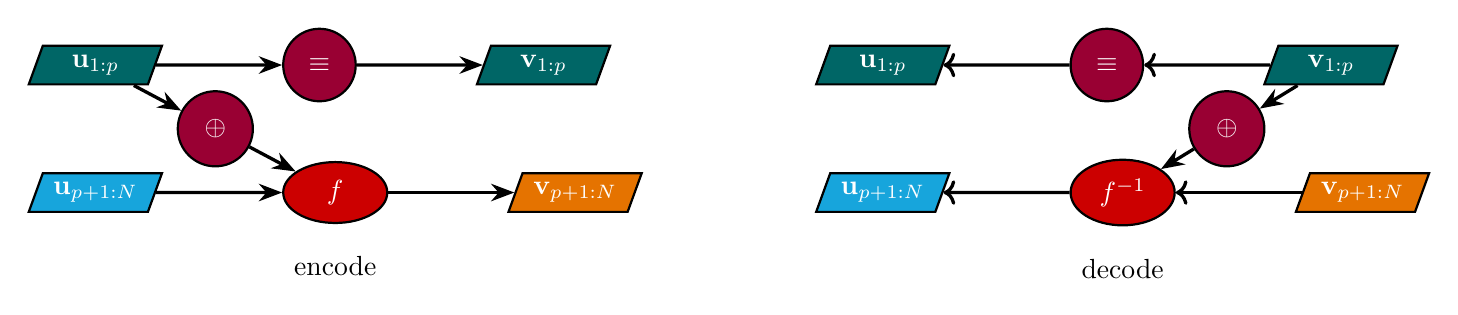
\begin{tikzpicture}[
    thick,
    node distance=16mm,
    data/.style={draw, trapezium, trapezium left angle=70, trapezium right angle=110, fill=teal!80!black, text=white, text width=11mm, align=center},
    proc/.style={draw, ellipse, fill=red!80!black, text=white, text width=7mm, align=center},
    op/.style={draw, circle, fill=purple!80!black, text=white, text width=6mm, align=center},
    arr/.style={-Stealth, line width=1.2pt, color=black}
  ]

  % Forward Flow
  \node[data] (inputA) {$\vec{u}_{1:p}$};
  \node[op, right=of inputA] (eqA) {\raisebox{-1ex}{$\equiv$}};
  \node[data, right=of eqA] (outputA) {$\vec{v}_{1:p}$};
  \draw[arr] (inputA) -- (eqA);
  \draw[arr] (eqA) -- (outputA);

  \node[data, below=1.1 of inputA, fill=cyan!90!black] (inputB) {$\vec{u}_{p+1:N}$};
  \node[proc, right=of inputB] (funcF) {$f$};
  \node[below=0.8em of funcF, anchor=north] (descF) {\textcolor{black}{encode}};
  \node[data, right=of funcF, fill=orange!90!black] (outputB) {$\vec{v}_{p+1:N}$};
  \draw[arr] (inputB) -- (funcF);
  \draw[arr] (funcF) -- (outputB);

  \node[op] (mergeF) at ($(inputA)!0.5!(funcF)$) {$\oplus$};
  \draw[arr] (inputA) -- (mergeF);
  \draw[arr] (mergeF) -- (funcF);

  % Inverse Flow
  \begin{scope}[xshift=10cm]

    \node[data] (inputC) {$\vec{u}_{1:p}$};
    \node[op, right=of inputC] (eqB) {\raisebox{-1ex}{$\equiv$}};
    \node[data, right=of eqB] (outputC) {$\vec{v}_{1:p}$};
    \draw[arr,<-] (inputC) -- (eqB);
    \draw[arr,<-] (eqB) -- (outputC);

    \node[data, below=1.1 of inputC, fill=cyan!90!black] (inputD) {$\vec{u}_{p+1:N}$};
    \node[proc, right=of inputD] (funcG) {$f^{-1}$};
    \node[below=0.8em of funcG, anchor=north] (descG) {\textcolor{black}{decode}};
    \node[data, right=of funcG, fill=orange!90!black] (outputD) {$\vec{v}_{p+1:N}$};
    \draw[arr,<-] (inputD) -- (funcG);
    \draw[arr,<-] (funcG) -- (outputD);

    \node[op] (mergeG) at ($(outputC)!0.5!(funcG)$) {$\oplus$};
    \draw[arr] (outputC) -- (mergeG);
    \draw[arr] (mergeG) -- (funcG);

  \end{scope}

\end{tikzpicture}
\end{document}